\documentclass[twoside,english]{uiofysmaster/uiofysmaster}

\usepackage[toc,titletoc,title,page]{appendix} %to add appendices (and have them in toc)
%\usepackage{mhchem} %latex chemistry symbols
\usepackage{blindtext} %to fill in dummy text
%\usepackage{cite} %to have multiple citations in one \cite{key1,key2,..} -do not use with natbib!!
\usepackage{tcolorbox} %to have boxes w color around text and math mode
\usepackage{enumitem} %to reduce vertical spacing in enumerate
\usepackage{tabu} % to set tables to page width
%\usepackage{aas_macros}
\usepackage{subcaption}
\usepackage{float}

\usepackage[sort&compress,square,comma,numbers]{natbib} %to use \citet, now mixed with [nr]
\usepackage[nottoc]{tocbibind}

%chapterlayout


\interfootnotelinepenalty=10000 % to force footnotes to NOT run over to the next page

%---
% to reduce space around table of contents (to fit everything into one page): 
\usepackage{tocloft}
\setlength{\cftbeforetoctitleskip}{0pt}
\setlength{\cftaftertoctitleskip}{0pt}
%---

\usepackage{epigraph}
\setlength\epigraphwidth{11cm}
\setlength\epigraphrule{0pt}

%---
\newcommand{\Cu}{${}^{64}$Cu} % making it faster to write Os192
\newcommand{\Osreac}{${}^{192}$Os$(\alpha$, $\alpha ' \gamma){}^{192}$Os}
\newcommand{\Osreacto}{${}^{191}$Os$(n$, $\gamma){}^{192}$Os}
\newcommand{\betadecay}{$\beta$-decay} % making it faster to write 
\newcommand{\bref}{B$^2$FH} % making it faster to write 
\newcommand{\gsf}{$\gamma$-strength function}
\newcommand{\ga}{$\gamma$}

%---
% modifying color in code listings and some style
\usepackage{color}
 
%\definecolor{codegreen}{rgb}{0,0.6,0} % too flashy
\definecolor{codegreen}{rgb}{0.0, 0.42, 0.24} % less flashy so comments not take all attention
\definecolor{codegray}{rgb}{0.5,0.5,0.5}
\definecolor{codepurple}{rgb}{0.58,0,0.82}
%\definecolor{codepurple}{rgb}{1.0, 0.0, 0.22} %carminered, could try it 
%\definecolor{backcolour}{rgb}{0.95,0.95,0.92} % original suggestion
\definecolor{backcolour}{rgb}{0.94, 0.97, 1.0}% aliceblue, not so flashy and not as ugly
 
\lstdefinestyle{mystyle}{
    backgroundcolor=\color{backcolour},   
    commentstyle=\color{codegreen},
    %commentstyle=\color{codegray},    
    keywordstyle=\color{magenta},
    numberstyle=\tiny\color{codegray},
    stringstyle=\color{codepurple},
    basicstyle=\footnotesize,
    breakatwhitespace=false,         
    breaklines=true,                 
    captionpos=b,                    
    keepspaces=true,                 
    %numbers=left,     %removing line numbers in the code snippets               
    %numbersep=5pt,                  
    showspaces=false,                
    showstringspaces=false,
    showtabs=false,                  
    tabsize=2,
    %float=tp,
    %floatplacement=tbp
}
 
\lstset{style=mystyle}
\renewcommand{\lstlistingname}{Code}
%---

%---
% new tcolorbox environment
% #1: tcolorbox options
% #2: color
% #3: box title
\newtcolorbox{mybox}[3][]
{
  colframe = #2!25,
  colback  = #2!10,
  coltitle = #2!20!black,  
  title    = #3,
  #1,
}

%---


%\bibliography{references}

\author{Nora Irene Jensen Pettersen}
\title{Cross-section meassurements for  $^{nat}Zn(n,p)64,67Cu$ reaction
%\title{Nuclear impact on astronomical processes: a first experimental constraint on the s-process $^{191}$Os$(n,\gamma)$ reaction rate %for the s-process in AGB stars
%\title{Nuclear impact on astronomical processes: benchmarking indirect measurements of s-process reaction rates for \Os 
}
\date{August 2020}
 
% ----------------------------------------------------------------------------------------------------------------------
% ----------------------------------------------------------------------------------------------------------------------
%Equations
%
%The command \eqref{} works exactly like \ref{}, but it adds parantheses to a plain number.
%
%Figures and tables
%
%\autoref{} is a usefull command when refering to to figures and tables. The command creates a reference with additional text corresponding to the target's type. For example, the command \autoref{fig:myfigure} would create a hyperlink to the \label{fig:myfigure} command, wherever it is. Assuming that this label is pointing to a figure, the hyperlink would contain the text "Figure 1.1", or similar.

%Two basic citation commands, \citet and \citep for textual and parenthetical citations, respectively. …
%\citet{jon90} --> Jones et al. (1990)
%\citep{jon90} --> (Jones et al., 1990)
%\citet*{jon90} --> Jones, Baker, and Williams (1990)
%\citep*{jon90} --> (Jones, Baker, and Williams, 1990)


\begin{document}

% set space around equations
\setlength{\belowdisplayskip}{12pt} \setlength{\belowdisplayshortskip}{12pt}
\setlength{\abovedisplayskip}{12pt} \setlength{\abovedisplayshortskip}{12pt}

\maketitle

%Centering the front page, see: https://github.com/ComputationalPhysics/uiofysmaster

\begin{abstract}
%An abstract summarizes, usually in one paragraph of 300 words or less, the major aspects of the entire paper in a prescribed sequence that includes: 1) the overall purpose of the study and the research problem(s) you investigated; 2) the basic design of the study; 3) major findings or trends found as a result of your analysis; and, 4) a brief summary of your interpretations and conclusions.


%However, it is difficult to conclude on the significance of the result.


\end{abstract}

\begin{dedication}
  %Til min kjære
  For me
  \\\vspace{12pt}
  %This is in dedication to 
  DEDICATION TO
    % To my dear oppvaskmaskin. Du vet hvem du er. 
    
  
\end{dedication}



\begin{acknowledgements}
THANK YOU

  \vspace{1.5cm}
  
  \noindent\textit{Nora Irene Jensen Pettersen}\\
  
  \noindent DATO
  
\end{acknowledgements}

\tableofcontents

% ----------------------------------------------------------------------------------------------------------------------
% ----------------------------------------------------------------------------------------------------------------------


\chapter{Introduction}

\epigraph{\itshape ``Count only the good days."}{--- \textup{ Irene Jensen}, Ahus 2017}
 
% Abbe G. Lemaitre (Observatory, Louvain), Nature 1931


%Cancer. It can happen to us all, whether we like it or not. We all know someone or know someone who knows someone with cancer or had died of cancer. It sucks. But what if. What if there was a way to get rid of it? A tumor inside you, that grows without you knowing it. It can take years without you knowing it is there, and when you feel it, it might be too late. With regular radiation you will have that risk of radiate healthy cells and damage them, and over time they can become new cancer cells which can kill you all over again. That is why I want to look into this kind of radiation, where you radiate from the inside and out. Where you don’t damage to many healthy cells but only the bad ones. This type of radiation can reach places in the body where regular radiation will not, in the brain and deep under the skin. A patient with brain tumor can not be radiated because that will also damage other part of the brain that the person needs, so why not send the radioactive molecule into the tumor itselfs? I would.







%SEC: a short history lesson and intro to astrophys/cosmo/nuc astro
%\section*{A short astronomical history lesson} 
\paragraph{A short introduction to nuclear medicine} \mbox{}
%\paragraph{A short astronomical history lesson} \mbox{}

\noindent
The usage of medical radionuclides can be traced back as long as late 1890s when Henry Becquerel discoverd radioactivity when he was studying a sulfate of uranium and Marie Curie together with her husband, Pierre Currie, forund activity in the ore where they had extracted uranium from. Since then, many studies on animal and humans have been done which led to development of radionuclides used in therapy and imaging with radiotracers.
\\ 
\\
Therapeutic application involves using radioisotopes together with a molecule or proteins to e.g. irradiate cancer cells. The advantage of this treatment method is that the biological molecules are being produced for one purpose only, to find a specific area in the body and irradiates it from the inside unlike external beam therapy. This approach is also used in diagnostics. A PET-scan makes an image of the activity in vivo, this imaging technique is commonly used to detect cancer, heart problems and brain disorders with the usage of different molecules.
\\
\\
In this report, medical isotopes are being discussed. The usage of radiopharmaceuticals in both therapy and diagnostics are used more and more in hospitals to treat and detect illnesses. The characteristics of a medical isotope and why those are important aspects is described in the first part of this report. The second part gives an introduction to different production methods of medical isotopes and the final part of this report is the usage of these radiopharmaceuticals.  
\\


% ----------------------------------------------------------------------------------------------------------------------
% ----------------------------------------------------------------------------------------------------------------------

\chapter{Theory}
\label{ch: beyond}

\epigraph{\itshape quote}{--- \textup{by}, }
 


\section{Background of Nuclear medicine}
\label{sec:Background}

According to the National cancer institute \cite{history_medicine} there were 1.735.350 people diagnosed with cancer in 2018 in the United States alone. The amount of deaths caused by cancer worldwide is approximate 9.6 million people \cite{WHO}. If we did not have modern medicine like chemotherapy and internal and external radiation, the number of deaths would be much higher. 
\\
\\
From when radioactivity were discovered in the 1890s there were a lot of new findings done in the medicine field, such as x-rays by Roentgen in 1895. Not long after, the biological foundation of nuclear medicine followed \cite{Cherry2012_chap1}. The tracer approach was developed in 1913 by Georg de Hevesy \cite{Hevesy2014} when he was investigating the absorbtion of radioactive led in plants. Not much later, in 1927, Blumgart and Weiss \cite{Blumgart1927} used aqueous solution of radon to study the pulmonary circulation \footnote{Pulmonary circulation is the portion of the circulatory system that carries deoxygenated blood from the right side of the heart to the lungs, where the blood oxygenates and returns to the left side of the heart.} in a man. Then, a cyclotron was build. Ernest Lawrence build the first cyclotron in Berkeley with the intention of accelerating particles to a high enough energy so they can be used to produce new particles \cite{E.Lawrence}. From a German article written by Winder$\ddot{o}$e on multiple acceleration on a positive ion Lawrence got the idea that he could make the particle reach a high enough energy by using a magnetic field such that the particle would bend and go around in a circle, and for each round in the circle the particle would increase its energy. It was his brother however, John, who realized that this can be used in medical applications. John was a medical doctor and was interested in the usage of radioisotope to treat cancer and in 1935 he came to Berkeley to do some testing on mice witch had a positive outcome. In 1937 John moved to Berkeley and performed his first treatment on a human using radioisotope, in fact Ernest and Johns mother got diagnosed with cancer in her uterus with a few month to live. John and Ernest got her to a special clinic that treated her with radiation and she lived for another 15 years \cite{E.Lawrence}. 
\\
\\
In the 1950s,  positron emitters and their usage in imaging tequnics were described by Frank R. Wrenn, Myron L. Good and Philip Handler \cite{Wrenn1951}. This opened up to the posibility to use radioactive isotopes together with a discover and diagnose different diseases. The mainly used radionuclide that was used before the discovery of $^{99m}Tc$ in 1964 \cite{harper_tc99m} was $^{131}I$ and was used to study and diagnose thyroid dissorders \cite{Cherry2012_chap1}. After Paul Harper and his colleagues used $^{99m}Tc$ for brain scanning \cite{harper_tc99m},  because of its flexibility for labeling, $^{99m}Tc$ was being used to study varies of organs in the body. The gamma property of $^{99m}Tc$ was proven to be good for imaging, and the fact that it could be produced in a long-lived generator made it attractive for usage in hospitals \cite{harper_tc99m}. One other big developent was the mathematics to produce an image of a body based on angular views around the patient \cite{Cherry2012_chap1}. This technique was important for the evolution of nuclear imaging, and are the basis for imaging procedure that is being used today like SPECT, CT, MRI and PET.
\\
\\
Today, nuclear medicine is used for both diagnostics and treatment of a patient. PET and SPECT is two imaging techniques that are most used in diagnostics. $^{18}F$ is the most used radionuclide in PET scans. Attached to a sugar molecule it will find cacerous cells in the body. In SPECT scans, $^{99m}Tc$ is often used to diagnose Coronary artery diseases and storke. These two illnesses are the number one killer worldwide and $^{99m}Tc$ is therefore the moste widely used radioisotope. Near 80 $\%$ of all procedures are using $^{99m}Tc$. In therapy, the radioisotope that is being used depends on the illness to the patient. What type of radionuclide that is being used in both diagnostics and therapy depends on the characteristics of the isotope.   
\\
\\

\section{Characteristics of medical radionuclides}
\noindent
\\
Radionuclides for therapeutic and diagnostic use have three principle factors that affect the ability for it to preform as a medical isotope in medicine\cite{invivo}, biological-, physical-, and chemical properties.\\
The biological and chemical feature involves the stability in a living organism, biological half-life, toxicity, tissue targeting and retention of radioactivity in the tumor\cite{Yeong}.
The physical characteristics include physical half-life, energy of the radiation, purity of the radionuclide, type of emission, daughter product(s) and method of production\cite{Yeong}. \\
\\\\
In this section, a book by Krane\cite{Krane} is used to describe the general nuclear reactions.\\



\subsection{Half-life}
The physical half-life, $t_{1/2}$, of a radioactive substance is the time it takes for a given amount to be reduced by half as a consequence of its decay and is described by the formula $$N(t) = N_0e^{-\lambda t} $$ 
where $N_0$ is the amount of initial substance, N(t) is then how much there is left after time, t, and $\lambda$ is the decay constant. This equation can be solved and the half-life of the decaying quantity is then given as $$t_{1/2} = \frac{ln2}{\lambda}$$ \\
\\
When a radioactive pharmaceutical gets injected into a human body, the biological half-life is important. It is the time it takes for a living body to reduce a biological substance by half through its biological processes. Therefore, when a radiopharmaceutical is produced to be used in a patients body, this is something that has to be considered carefully. It should be long enough to do a procedure, but short enough to not damage unnecessary healthy tissue. \\
\\
In diagnostic, the half-life should only be a few hours. From when the radioisotope is produced it starts to decay, and it is important that the half-life is long enough such that it can be used. If a patient is taking a PET-scan, depending on the radionuclide, a procedure using $^{18}F$ usually takes 30-60 minutes to execute. Therefore, the radiopharmaceutical have to have a half-life longer than it takes from production of the radioactive substance to the end of the procedure.
\\
\\
For a therapeutic isotope, it should have a half-life of approximately a few days. It should be long enough to deliver the right amount of dose to the area of interest. But the most important factor is the effective half-life, that is both physical and biological half-life within a patients organ\cite{Yeong}. The physical half-life is well known, but the biological half-life is dependent on several things, like what kind of tracer is being used, metabolism, uptake and how the pharmaceutical leaves the body\cite{Yeong}.\\
It depends on the uptake mechanism, type of tumor and method of administration\cite{Yeong} on what kind of tracer and isotope that should be used. If the patient has a low uptake, the physical half-life should be longer such that it will not emit radiation before it has reached the tumor, but not too long such that it sends out radiation on its way out of the body. 
\\
\\
Travel time is also a factor when choosing an isotope. Based on the physical half-life, some hospitals can produce some radioisotopes themselves. If they have a cyclotron in the hospital they can produce some isotopes, such as $^{18}F$ with half-life of 109 minutes, that is used in PET scans. In those cases the half-life can be shorter than if it has to be transported to another part of the county. \\
\\

\subsection{Stopping power}
When a charged particle penetrates an absorbing medium it will slowly slow down due to energy loss, the parameter that describes this is called stopping power. There are two known cases of stopping power\cite{Nuclear_medicine}, collision, $S_{col}$, and radiative, $S_{rad}$, stopping power. $S_{col}$ is a result from charged particles interaction with orbital electron of the material while $S_{rad}$ is when the charged particle interact with the nuclei in the material. The total stopping power is $S_{tot} = S_{col} + S_{rad}$ \\
\\
Electrons can lose energy by Bremsstrahlung and by ionization. At high energies where a particle travels faster than the speed of light in a medium, Cherenkov radiation happens. This is an important phenomena but the energy loss in this process is small\cite{nuclearchem}.\\
\\
Even though the majority of the energy loss for electron is by collisions, the emission of bremsstrahlung photons is also important. When an electron is traveling close to an atomic nucleus it can decelerate due to the Coulomb field of the nucleus and atomic electrons. When this happens, the electron will transfer energy to a photon that gets emitted. When the kinetic energy of the electron increases the yield of bremsstrahlung increases.
\\
\\
When it comes to photons, the beam intensity I(x) will decrease with \begin{equation}
    I(x) = I_0e^{-\mu x}
\end{equation}
\noindent
where $\mu$ is the attenuation coefficient and are dependent of the energy h$\nu$ of the photon and the atomic number Z of the absorber\cite{Nuclear_medicine}. $I_0$ is the initial intensity of the beam at depth in medium where x = 0.\\
\\
Photons will also interact with a medium through photoelectric effect, Compton scattering and pair production, these are briefly discussed in section 2.1.3 under $\gamma$ and X-rays.\\
\\
\\
\noindent
\textbf{LET}\\
For therapy, the biological effect depends on how the isotopes decay, and how it distributes its energy to the surrounding medium. High linear energy transfer (LET) will concentrate the deposited energy to a small area near its tracks, as a result the biological damage is grater and there will be more damage to the DNA and other cellular structure. LET is closely related to the linear energy loss $\frac{dE}{dx}$ except that LET does not include radiative losses of energy. \\
\begin{figure}[h]
    \centering
    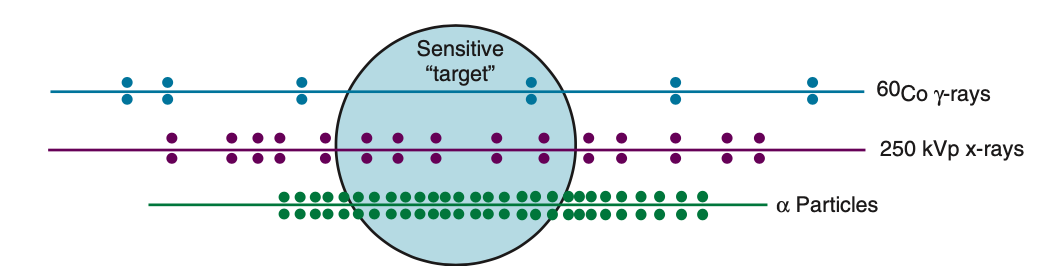
\includegraphics[scale=.4]{low_vs_high_LET.PNG}
    \caption{An illustration from \cite{Zeman2015_chap1} of low LET vs high LET}
    \label{fig:higvslowLET}
\end{figure}
\\
As shown in figure \ref{fig:higvslowLET}, high LET will do more damage in a smaller area and the therapeutic effect is significantly better than for low LET. $\alpha$ is a nuclei with high LET. \\
Low LET, as figure \ref{fig:higvslowLET} shows, is when the particle distribute little ionization throughout the medium, which results in little to no damage on the cells along the way. In diagnostic, we want to use isotopes that decays with particles who follows low LET and the opposite for therapy.\\
\\
Since the ionization of a material increases when the energy decreases for particles\cite{Nuclear_medicine}, the radiation will be more significant at the end of its tracks. Figure \ref{fig:braggcurve} shows how the ionization alters as the particle goes through a medium. The peak at the end is the bragg-peak and is correlated with high LET where most of the ionization happens at the end of its range. 

\begin{figure}[h!]
    \centering
    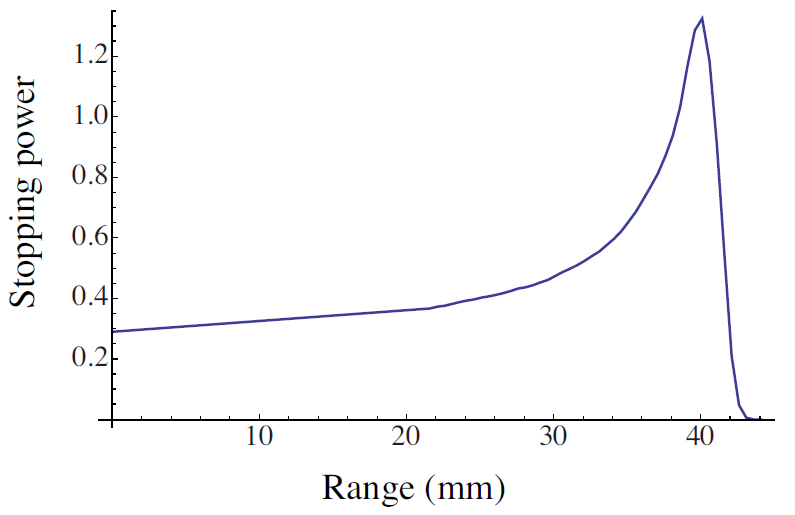
\includegraphics[scale=.25]{bragg.png}
    \caption{Illustration of the bragg curve for charged particles. Picture from \cite{inbook}}
    \label{fig:braggcurve}
\end{figure}


 
\section{Decay modes}
\label{sec:decaymodes}

When a patient have to go trough diagnostic and therapy with radioisotopes, the isotopes that is being used have do undergo decay that gives the wanted radiation. For therapy, decay modes  that gives a $\gamma$ or $e^{+}$ is important. In therapy, the wanted decay mode gives off an $e^{-}$, $\alpha$ and smetimes $\gamma$.

\subsection{$\beta$-decay}

Decay by $\beta$ can happen by $\beta$-, EC (see auger electrons) or $\beta$+ decay.\\
$\beta$-:
\begin{equation}
n \rightarrow p + e^- + \bar{\nu_e} 
\end{equation}\\
$\beta+$:
\begin{equation}
p \rightarrow n + e^+ + \nu_e
\end{equation}\\
For therapy, $e^-$ will travel longer in a medium than $e^+$ (will annihilate fast).\textcolor{red}{WHY?} $e^-$ will ionize matter on its path and we want to take advantage of that. Therefore, it is $\beta$- decay we are interested in when we treat a patient. $\beta$+ decay are used in diagnostic. If we want to take a picture of the biological activity in a patient, $e^+$ is the source of interest for usage of PET scans, which I will discuss in section 4.1.\\
\\
Compared to $\alpha$ particles, $\beta$ particles travels a lot further and creates less ionization to the surrounding medium on its path. This is important when the biological effect matters. There are however, difference in the range of various of isotopes that undergo $\beta$ decay. Short range $\beta$-particle emitters have a relatively short range, a couple of $\mu m$, in tissue that is suitable for treatment of small tumor metastases%\cite{nuclearchem}. 
The $\beta$-emitters with long range in tissue can penetrate with an average of more than 2 mm and can be used to treat i.e. rheumatoid arthritis, which is an autoimmune disorder that often affect joints.\\
\\
The energy of $\beta$ particles are not distinct, but rather more spread out in a spectrum.

%\begin{figure}[h!]
   % \centering
    %\includegraphics[scale=0.4]{betadecay.png}
    %\caption{A typical illustration of the energyspectra for beta decay. From \cite{medical}}
    %\label{fig:beta_decay_energyspec}
%\end{figure}

The spectrum in figure %\ref{fig:beta_decay_energyspec} 
shows how the energy are divided between the electron and the anti neutrino. The electrons of beta particles will interact with the surrounding electrons by dismissing the it from its orbit and producing a ion pair or cause excitation. Since the amount of damage tissue is related to LET and $\beta$ particles penetrates further in to a medium than $\alpha$ particles, $\beta$ particles has lower LET than $\alpha$ does. Exposure to $\beta$ results therefore in less damage.\\
\\
$^{90}Y$ is one popular long range isotope used in therapy, it has a mean range of 3.900 $\mu m$ and an average energy of 935 KeV%\cite{nuclearchem}
, while a widely used short range beta emitter is $^{131}I$. It has a mean range of 910 $\mu m$ and an average energy of 182 KeV%\cite{nuclearchem}.
 The energy will vary from almost zero to the maximum energy, and the average energy is approximately one third of the maximum energy. For therapy, the mean energy dependent mean and maximum range in tissue for beta emitters. 
\\
\\

\subsection{Electron capture, Internal convention and Auger electrons}

When low-energy X-ray photons collides with an atom and electron from the inner shell can get ejected. If the nucleus has too many protons, the electron can be captured by the nucleus where the electron and a proton turns into a neutron. This is called electron capture (EC). When this happens, there will be an empty spot in the K shell which one of the electrons in the L shell will try to fill. There will therefore be a vacancy in the L shell. This process releases an energy of $E_K - E_{L}$ and can be transferred to another electron in the L shell, resulting in ejecting it from the atom. This electron is called auger electron. It is a low energy electron that will have a kinetic energy of $T = E_k - E_{L1} - E_{L2,3}$ \cite{medical}, where $E_k - E_{L1}$ is the difference in binding energy. It has a short range and will deposit all of its energy in a highly localized site. The distance the auger electrons travels from <0.5 $\mu$m to a few nm in biological tissue \cite{augerelectrons}, it follows high LET and will therefor do a lot of damage to the DNA and other important structure in the cell nucleus that are important for the cell to live. Auger electrons are highly effective for killing these structure and breakage of double DNA strands due to its energy deposit in a short distance (see figure \ref{fig:auger}).\\
%\begin{figure}[h!]
%\centering
%\begin{subfigure}{.43\textwidth}
  %\centering
  %\includegraphics[width=.7\linewidth]{1200px-Auger_Process.jpg}
  %\caption{Illustration of emission of an auger electron, illustration from Wikipedia}
  %\label{subfig:augerlevel}
%\end{subfigure}%
%\begin{subfigure}{.43\textwidth}
  %\centering
  %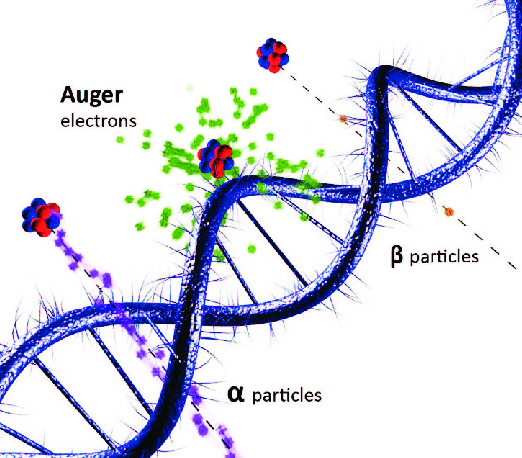
\includegraphics[width=.7\linewidth]{auger.png}
  %\caption{Range of auger electron compared to $\alpha$ and $\beta$ particles, taken from \cite{auger}}
  %\label{subfig:DNA}
%\end{subfigure}
%\caption{A description of auger electron}
%\label{fig:auger}
%\end{figure}
\noindent
\\
One other way auger electrons are created is due to the effect of internal conversion (IC). This is when an electron get knocked out of the inner shell and one other electron from a higher orbital jumps down to the inner shell. In this process energy gets realised by photons which can knock out an electron from the outer shell, the auger electron. 
\\
\\


\subsection{$\gamma$-decay and X-rays}

\textbf{$\gamma$ and X-rays interaction with matter}\\
\\
\noindent
Emission of $\gamma$-rays are usually a product from the radioactive decay of atomic nuclei. If the nucleus is left in an excited state, it will de-excite by either emit a photon.\cite{nuclearchem}. $\gamma$ decay are described as $$^{A}_{Z}X^* \rightarrow ^{A}_ZX + \gamma$$
where the excitation energy is transferred to a $\gamma$ photon plus the recoil energy.\\
\\
If the notation includes a "m" $$^{Am}_ZX \rightarrow^{A}_ZX + \gamma$$
in that case, the nucleus is in an isomer state where it is long-lived $(T_{1/2} < 1 \mu s)$ in an excited state\cite{nuclearchem}. The transition will then be described as an isometric transition (IT).\\
\\
Competing with $\gamma$-ray emission, internal conversion (IC) is a way for the nucleus to de-excite. It will electromagnetically interact with a shell electron witch leads to emitting of the orbiting electron\cite{toxicology}.\\
\\
\\  
X-rays, as $\gamma$-rays, are electromagnetic radiation. The difference is that X-rays has its origin outside of the nucleus. When X-rays and $\gamma$ penetrates a medium it can create different effects in the body by ionization.
Photoelectric effect, Compton effect and pair production. \\
\\
\begin{figure}[h!]
    \centering
     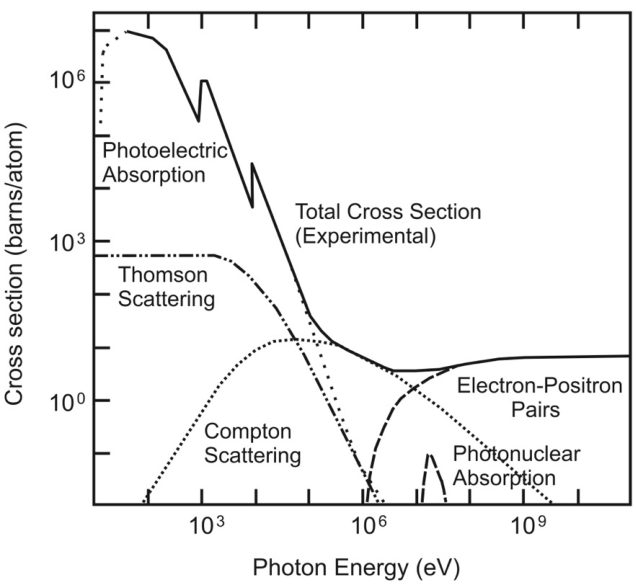
\includegraphics[scale=0.4]{pcp_cross.png}
     \caption{Cross section for photoelectric effect, Compton scattering and pair production. Taken from \cite{photoelectric_cross} }
    \label{fig:photo-compton-pair}
\end{figure}
\\
The photoelectric effect happens when a nucleus absorbs the incoming photon. The energy absorbed will be used to ejected an orbiting electron from the atom. This electron is called a photoelectron\cite{nuclearchem}. The electron cannot be emitted if the incoming photon energy is lower than the binding energy of the shell to the electron. The energy of the electron emitted is then $E_e = hv - E_b$. The probability of photoelectric effect happens is measured as the cross section 
$$\sigma = constant \cdot \frac{Z^n}{E^3}$$
where n is equal to 4 or 5\cite{Radiological_physics}. The photoelectric effect will increase with the atomic number and by that reason we are using lead (Z=82) as shielding for gamma radiation.\\ 
\\
Compton effect is scattering of a photon due to an electron. When an incident photon interacts with an atomic or free electron, it will bend from its original path with an angle $\theta$. The electron are then being emitted with an angle of $\phi$.\\
The energy is shared between the emitted electron and the photon, where the incident photon will transfer some of its energy to the electron. The final photon energy is $$h\nu' = \frac{h\nu}{1 + \frac{h\nu}{m_ec^2} (1-cos\theta)}$$
The atomic cross section is $$\sigma_a = Z \sigma_e$$ where $\sigma_e$ is the electronic cross section, assuming a free electron\cite{nuclearchem}.\\
\\
The last main effect is pair production. The incoming photon disappears, and spontaneously turns into an electron-positron pair. This can only happen if the energy of the photon is greater than the total rest mass of an positron-electron pair, 1.022 MeV. Since X-rays and $\gamma$ can penetrate long distances without ionizing the medium, emerges from the body and has a low LET, they are at good use for diagnostic of a patient with different imaging technique. \\
The cross section of pair is production is dependent on $Z^2$ .
\\
\\
Figure \ref{fig:photo-compton-pair} shows how the three main interaction of a photon is dependent on energy. For lower energies it is clear that the photoelectric effect is dominant, pair production is more probable to happen in higher energies.\\
\\
\\
\textbf{$\gamma$ decay}
\\
\\
When a nucleus is being exited, either by the cration of a compaound nucleus, with a direct reaction or if a nucleus decays with one of the decay modes described in \ref{sec:decaymodes}, the nucleus will decay into its groundstate by emitting a $\gamma$-ray. This is illustrated in \ref{fig:67cu_decay}.

\begin{figure}[h!]
    \centering
     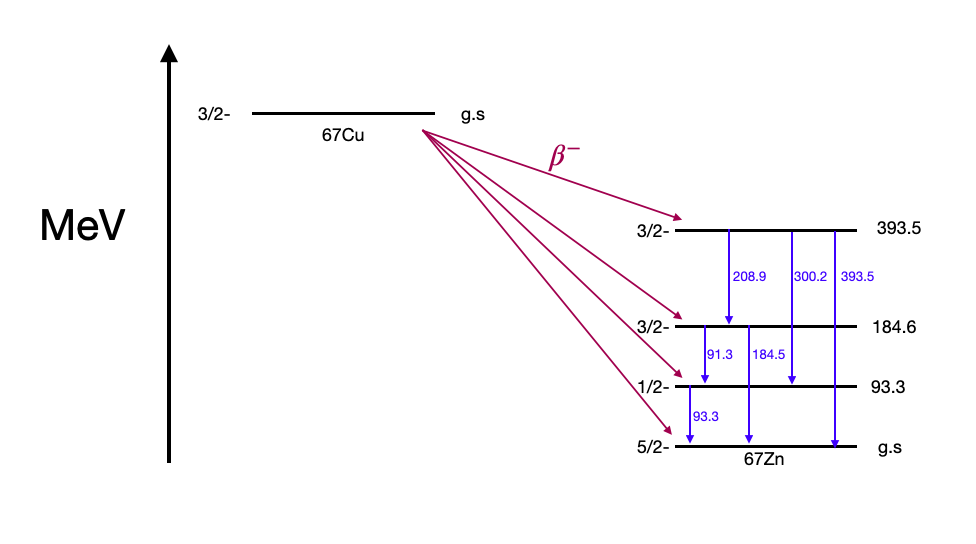
\includegraphics[scale=0.4]{67Cu_decay.PNG}
     \caption{An illustration on how $^{67}Cu$ is $\beta$-decaying down to $^{67}Zn$. } 
    \label{fig:67cu_decay}
\end{figure}
\noindent
As \ref{fig:67cu_decay} shows, the $\gamma$s that are emitted in $^{67}Zn$ when the nucleus deexite can have different energies. This depends on \textcolor{red}{what? why is 300 MeV more favourable than 393 MeV gamma? - Sunniva?}
\\
It is the $\gamma$-rays from $^{67}Zn$ that we are using to clame that $^{67}Cu$ were made, see \ref{ch:analyse}.


\section{Production of medical isotopes}
\subsection{Production rates and cross-sections}
\noindent
\textbf{Production rate}\\
\\
When there is a nucleon-nucleon interaction in a nuclei there will be change in the tribe of the nucleus and therefore the production of different nuclei can happen. This can happen by exciting a nuclei, exchange of nucleons or fusion. \cite{nuclearchem}\\
If a nucleus ends up in an excited state after a collision before it decays into a new nuclei, the states are described as \begin{equation}
    a + A \rightarrow C^* \rightarrow b + B 
\end{equation} \cite{nuclearchem}
where A is the target, a is the projectile, b is the light product and B is the new heavy product. If however, the nucleus doesn't get excited and decays into a new product, the general equation for a nuclear reaction is
\begin{equation}
    a + A \rightarrow b + B + Q 
\end{equation}
where Q is the reaction energy. The nuclear reaction is often written as $$A(a,b)B$$\\
\\
Equation 6 describes the creation of a compound nucleus, $C^*$. With low energies and a direct hit on the center of the nucleus gives the highest probability of creating a compound nucleus. When a direct reaction happens with higher energies and often at the edge of the nucleus, equation 7 defines this process\cite{Nuclear_medicine}. The production of radionuclides can therefore a mixture of these two reactions.
\\
\\
There are many ways as to which radionuclides can be produced. Neutron induced reaction, charged particle induced nuclear reaction, fission, selective separation and gamma induced are the most important ones\cite{Nuclear_medicine}.\\
\\
The neutron induced nuclear reaction can happen with a thermal neutron, where fission and (n,$\gamma$) is the production route, and with fast neutrons, where we can get (n,n'), (n,2n'), .., (n,p), .., (n,$\alpha$), and fission reactions. One advantage of using neutrons as a beam is that it can penetrate the target with quite low energies, in some cases it only needs an energy of 0.0025 eV to penetrate a nucleus\cite{Nuclear_medicine}. Charge particles however, needs to overcome the coulomb barrier to enter the nucleus. 
\\
\textcolor{red}{BILDE HER AV CROSS SECTIONS}
\\
\\
Charged particles can give rise to elastic-, inelastic- as well as other reactions. Elastic reaction is where the product before the collision is the same as the product after the collision, a (p,p) reaction. The masses, momentum and the kinetic energy before and after the interaction are identical\cite{Nuclear_medicine}.\\
Inelastic reaction, (p,p'), happens when energy is transferred to the product and the difference in kinetic energy is saved as excitation energy in the nucleus.
%\begin{center}
    %\begin{figure}[h!]
    %\centering
    %\includegraphics[scale=0.3]{production_cross_section.jpg}
    %\caption{The cross section of different nuclear reactons when $^{133}Cs$ is being irradiated with a neutron beam. Taken from \cite{neutron_reactions}}
    %\label{fig:nuclear-reactions}
%\end{figure}
%\end{center}
\noindent
Depending on the beam and energy, figure \ref{fig:nuclear-reactions} shows that there are different nuclear reaction channels that can happen. With higher energies, the outgoing particle can be heavier or more in number. 
\\
\\
\section{High purity Germanium detector}
\label{sec:ge-detector}

Most semiconductors are based on the n-p junction, which is a boundry between two different materials. A crystal is being doped on one side with a material that has one excess electron in the outer shell and therefore is called the negative side, or n-type. The other side is doped with a material that has one less electron in its outer shell, leaving a hole. This side is called p-type, since it is more positive. When these two types meet the electrons from the n-type will be attracted to the holes in the p-type and leaves a depletion zone in the middle of the crystal with a negative charge on the p-side and a positive charge on the n-side. This makes it hard for the electrons to travel to the p-side unless there is a voltage applied to the crystal. \\
\begin{figure}[h!]
    \centering
     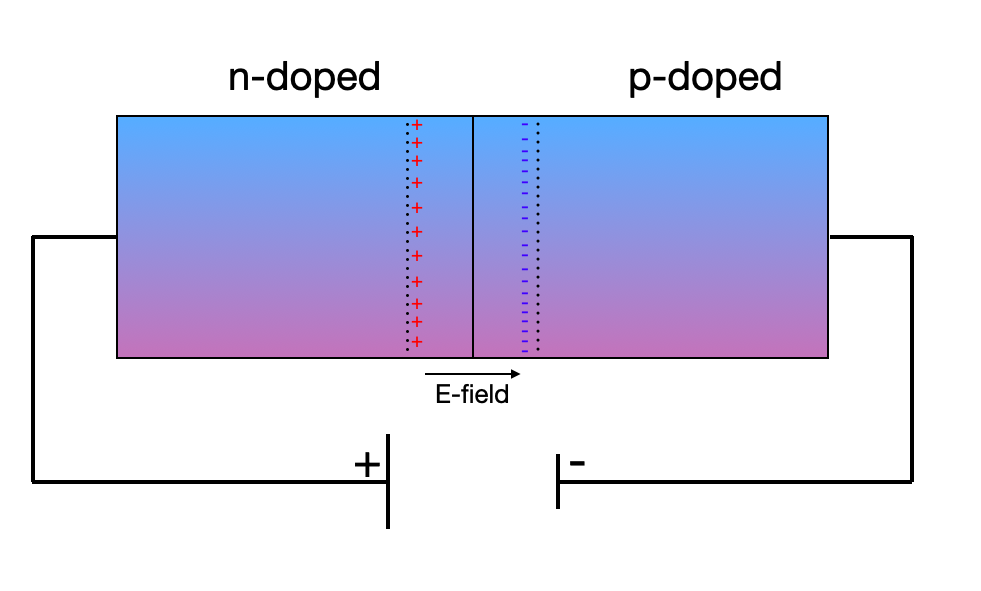
\includegraphics[scale=0.3]{semiconductor.png}
     \caption{n-p junction of a semiconductor} 
    \label{fig:n-p_junction}
\end{figure}
\noindent
\\
The effect of having an electric field is that  when you have a charge carrier being generated inside a region, the holes and the electrons will be pushed away and you get a depletion zone, a zone that doesn’t have a charged carrier in them. This can be used in different ways: If you don’t apply any voltage from the outside and the depletion zone will be quite small. The depletion zone can be used for detection, if you have a charge particle creating an electron hole inside the depletion zone the charge will be pushed out and you can (in principle) collect the charge outside of the depletion zone. However, charge that are created outside of the depletion zone can’t be collected because they will quickly recombine. So you have to implant and dope the same piece of material from different side. If we want to detect radiation we want to get a big depletion zone, we want as much as possible of the material detector to be depleted. This is done by reverse biasing.
\\
\\
\textbf{Reverse biasing} is done by applying an external voltage where a positive terminal is connected to the n-type side and a negative terminal to the p-type side. This will make the holes and electron to drift so the depletion zone become larger. The larger the voltage, the bigger the depletion zone unless too much voltage is applied. If you go too high in voltage you can cause the material to break down and damage the detector.
In an ideal case the detector will be a perfect isolator where there is no ions or photons being detected, but there can often be leaking current and that is because you can’t make it into a perfect isolator when you are not detecting anything. How much leaking that are coming out of the detector is a good indicator on how well it is functioning, a lot of leakage is bad. \textcolor{red}{WHY}\\
\\
The maximum depletion you can obtain is inversely related to the density of dopends. If a lot of dopend is added in the material to make it work, it means that there can only be achieved a smaller depletion zone. That’s why a pure material is needed. A pure material don’t need as much doping, less doping means that there can occure a thicker depletion thickness. That translates to having more material where you can detect particles and read out the deposit charge as pulses.
\\
\\
%For germanium detectros,
%If we compare the mean free path of photons in Si and Ge for 1000 KeV = 1MeV, you got a mean free path of 1 cm in Ge and several cm in Si. This means that if you want to detect 1 MeV photons you have a much better chance using Ge than Si. This is the main reasons that we use Si to detect charge particles and Ge or something with higher atomic number to detect photons. The excellent energy resolution you can obtain with Ge are also a reason that we use Ge detector.

Germanium detectors need to be cooled down to avoid leakage current due to thermal excitation. You can cool it down with air, but that is not as good as liquid nitrogen. With air you can get more thermal fluctuations, you are not able to get the same low temperature with the electrical air cooling. 
\\

\section{PET-scans}
\label{sec:PET}

Positron emission tomography (PET) is an imagining technique to measure the activity in the body by using radiotracers\cite{molecular_imaging}. PET uses annihilation photons that are produced when a positron interacts with an electron and thus, the radiotracers that are being used has to contain a positron emitter. \\
The basic principle of PET imaging is that when a positron merges with an electron in the body they will convert into two photons that will get released in the opposite direction with approximately 180 degrees between them\cite{physics_in_medicine}. The energy of the photons are identical (511 KeV) and will be detected by detectors that are placed around the patient. The observing of the photon is done by the principle of annihilation coincidence detection (ACD), this means that the detection of photons happens without collimator. This makes it possible to find their origin along a line between the detectors\cite{physics_in_medicine} as shown in figure \ref{fig:TOF_PET}.\\
\\

\begin{figure}[h!]
\centering
\begin{subfigure}{.5\textwidth}
  \centering
  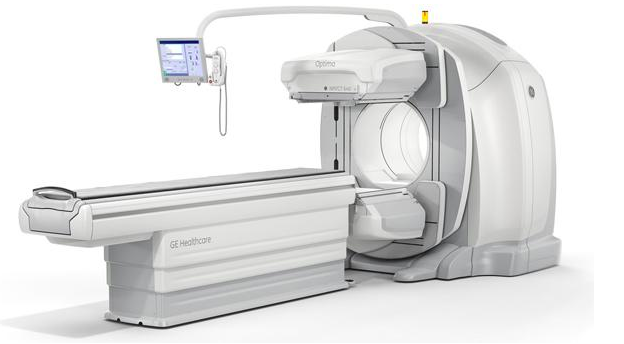
\includegraphics[width=.7\linewidth]{petscan.png}
  \caption{PET machine}
  \label{fig:PET}
\end{subfigure}%
\begin{subfigure}{.5\textwidth}
  \centering
  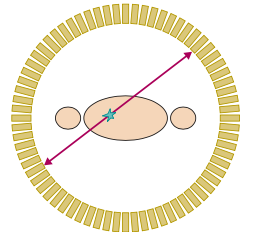
\includegraphics[width=.7\linewidth]{TOF_PET.png}
  \caption{How a photon travels to the detectors around the patient}
  \label{fig:TOF_PET}
\end{subfigure}%
\caption{Subfigure (a) shows a clinical PET that is used in hospitals and subfigure (b) visualizes the detection of photons. Both taken from \cite{physics_in_medicine}.}
\label{fig:PETSCAN}
\end{figure}
\noindent
\textbf{Applications of PET}\\
\\
The usage of PET scans requires an isotope that will emit a positron, and $^{18}F$ does just that. It has a half-life of 109 minutes and is the most common isotope used in PET. The uptake for fludeoxyglucose ($^{18}F$), or FDG in the tissue indicates that there is a pathological condition that increases the tissues metabolic rate\cite{physics_in_medicine}. The fact that FDG can be used for a whole body scan makes $^{18}F$ a favorite as a medical isotope. As figure \ref{fig:PET_breastcancer} shows, FDG-PET is a good imaging technique not only to detect cancer, but also find metastasis and to see how the treatment is working.\\ Combining PET with CT gives a more precise anatomical localization of the radioactive substance that is inside the body. 
\\
\begin{figure}[h!]
\centering
\begin{subfigure}{.5\textwidth}
  \centering
  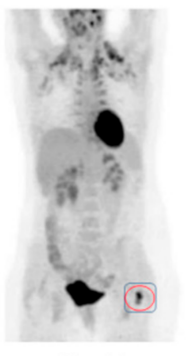
\includegraphics[width=.4\linewidth]{PET_breastcancer.png}
  \caption{FDG-PET scan of a 47-year-old woman with primary breast cancer, but as the PET scan shows, also metastasis in hip bone. Taken from \cite{PET_breastcanser}.}
  \label{fig:PET_breastcancer}
\end{subfigure}%
\begin{subfigure}{.5\textwidth}
  \centering
  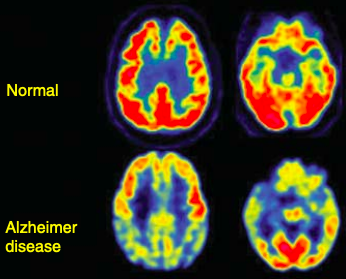
\includegraphics[width=.75\linewidth]{PET_alziemer.png}
  \caption{A FDG-PET scan of a brain with Alzheimer disease. Taken from \cite{PET_alzimer}.}
  \label{fig:PET_alzimer}
\end{subfigure}
\caption{Examples on what images from PET scans can look like.}
\label{fig:FTG-PET}
\end{figure}
\noindent
\\
$^{18}F$ can also be used in neuroimaging. The brain uses glucose as fuel and for this reason FDG-PET is not for imaging the brain. But, Alzheimers disease usually decrease the metabolic activity, leaving the brain with less oxygen and glucose \cite{18F_alzimer}. As shown in figure \ref{fig:PET_alzimer}, there are clearly less activity in the brain due to Alzheimer disease. FDG can aslo be used to find other neurodegenerative diseases, dementia, epilepsy, neurodevelopmental disorders and psychiatric disorders\cite{physics_in_medicine}.
% ----------------------------------------------------------------------------------------------------------------------
% ----------------------------------------------------------------------------------------------------------------------

\chapter{Cu64,67} 
\label{ch: mywork}

\epigraph{\itshape QUOTE.}{--- \textup{BY}}


\section{what can we do to make the nuclear medicine better?}
\label{sec: betterwork}

Nuclear medicine is a growing field within diagnostic and treatment of a patient. The usage of many different medical isotopes is being used to different illnesses, and there is always good to have new isotopes that can be used in nuclear medicine.\\
Nuclear medicin is being produced as a peronalized medicine. This indicates that the patients characteristics such as anatomy, physological and genetic are being evaluated when radioisotopes for diagnostic and therapy are being chosen \cite{Ahmedova2018}. 
\\
\\
To make the planning and excecution of a treatment easier and more efficient, researchers are looking at different ways to combine therapy and diagnostics. 
$^{64}Cu$ and $^{67}Cu$ are two theranostics isotopes that are interesting due to their half-life, decay scheme, 


 \begin{tabular}{  p{3cm} p{3cm} p{3cm} p{3cm} p{3cm}   }
 \hline
Isotope  & Half-life & Decay ($\%$) & Usage & Source \\
 \hline
 $^{64}Cu$ &  12.07 hours & $\beta$+ & Diagnostic: PET & Cyclotron \\
 $^{67}Cu$ &  2.57 days & $\beta$- (100) & Therapy: Tumor & Cyclotron \\
 \hline
\end{tabular}
\\
\\
\textcolor{red}{-medical prespecctive: we wan to introduce a new theragnostic pairs to use in hospitals\\
- how wonderful Cu64,67 are\\
-- properties\\
-- papers\\
-- better than a lot of the studff we are already using\\
-- motivation for my work\\
---- can adjust ratio for 64,67 Cu by tuning the energy of the beam}\\



\subsection{My motivation}
\label{sec: my_motivation}




\subsection{Physics motivation}
\label{sec: physics_motivation}

- cu64,67 are amazin but now, we have not a good way for making them. tell about my way of create them\\
-- deuterium breakup (n,-) way\\
-- how we are doing it\\


\section{Theranostic}
\label{sec:theranostic}
% ----------------------------------------------------------------------------------------------------------------------

% ----------------------------------------------------------------------------------------------------------------------

\chapter{The experiment}
\label{ch: experiment}

In this theses we wanted to study the $^{nat}Zn(n,x)^{64,67}Cu$ reaction. 
In the following chapter, the experiment in itself is being discussed. Sections 4.1.1, 4.1.2 and 4.1.3 describes the 88-Inch cyclotron used int the experiment, the deuterium breakup process and how the targets were stacked together before being irradiated.


\section{The experimental setup}
\label{sec: setup}

The experiment was preformed on August 2018 at the Lawrence Berkeley National Laboratory where a deuterium beam with an energy of 16 and 33 MeV was used. The deuterium was used in the purpose to hit a berillium target, creating a neutron beam. Five targets, zinc, zirconium, indium, yttrium and aluminum were then irradiated with the neutrons, for illustration see fig \ref{fig:D_to_n}. For the 16 MeV run, the targets were irradiated for 7 hours and 57 minutes, and 1 hour and 52 minutes for the 33 MeV run. The length of the irradiation is different since the energies are different. A higher energy beam and a longer irradiation time will increase the dose and open up for other production rates. Since the germanium detector that was used to count the foils after irradiation have a couple of nS of deadtime, there will be a lot of information lost if the 33 MeV run was longer than 1.52 hours. The activity would have been much higher and the detector would not had been able to cach all the activity.\\ When 33 MeV is used, we know from section \ref{sec: D_breakup} that the number of neutrons that are being produced in the prosses is two to three times higher than for 16 MeV. This is also a reason for the shorter irradiation time for 33 MeV.

\begin{figure} [H]
   \centering
   \includegraphics[height=.6\textheight, angle=90]{Control-Room-Map.pdf}
   \caption{Map over the 88-inch cyclotorne at Lawrence Berkeley National Laboratory\textcolor{red}{FROM?}}
   \label{fig:Control-Room-Map}
\end{figure}
\noindent
The irradiation took place in cave 0, see figure \ref{fig:Control-Room-Map}. In figure \ref{fig:Control-Room-Map} there is a green line, which is the beam line. For the beam to get to cave 0 it has to go throug two bending magnets where the deuterions with the highest and lowest energies will be lost when the beam are being bend to the right beamline. Cave 0 has good shielding and when high energy beam enters the cave there will be more x-rays in the room. Shielding is therefore one of the main reasons to why high energy experiments are being done in cave 0.


The beam had to be tuned such that it didn't have a lot of angular distribution before it hits the targets. The neutrons gets emitted from the beryllium target with an angular distribution and the targets are based on the energy the neutrons hitts the target with. The angle should be about zero degrees and the targets are therefore placed 10 cm back from the be disk. The targets will not be activated with the full beam energy and the intensity of the neutrons will decrease with distance-squared, x$^2$. \textcolor{red}{reference to where you talk about solid angle}

\begin{figure} [H]
\centering
\begin{subfigure}{.5\textwidth}
  \centering
  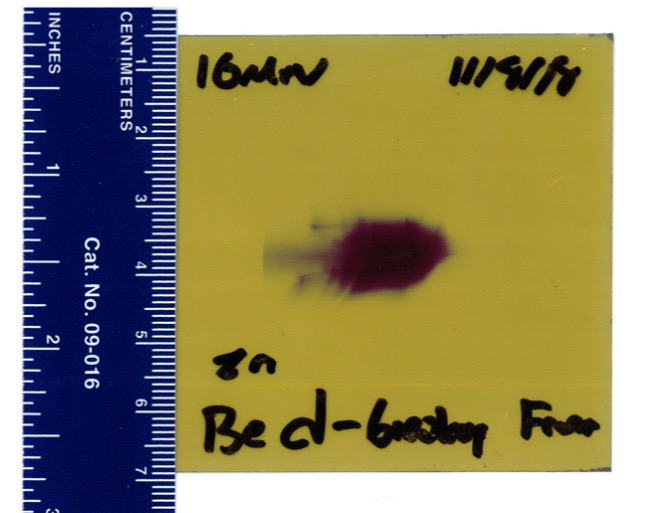
\includegraphics[width=1\linewidth]{16MeV_front.jpeg}
  \caption{A subfigure}
  \label{fig:sub1}
\end{subfigure}%
\begin{subfigure}{.5\textwidth}
  \centering
  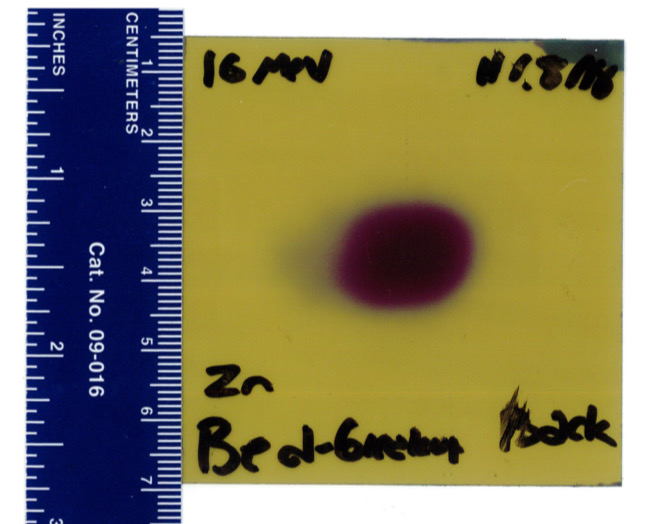
\includegraphics[width=1\linewidth]{16MeV_back.jpeg}
  \caption{A subfigure}
  \label{fig:sub2}
\end{subfigure}
\begin{subfigure}{.5\textwidth}
  \centering
  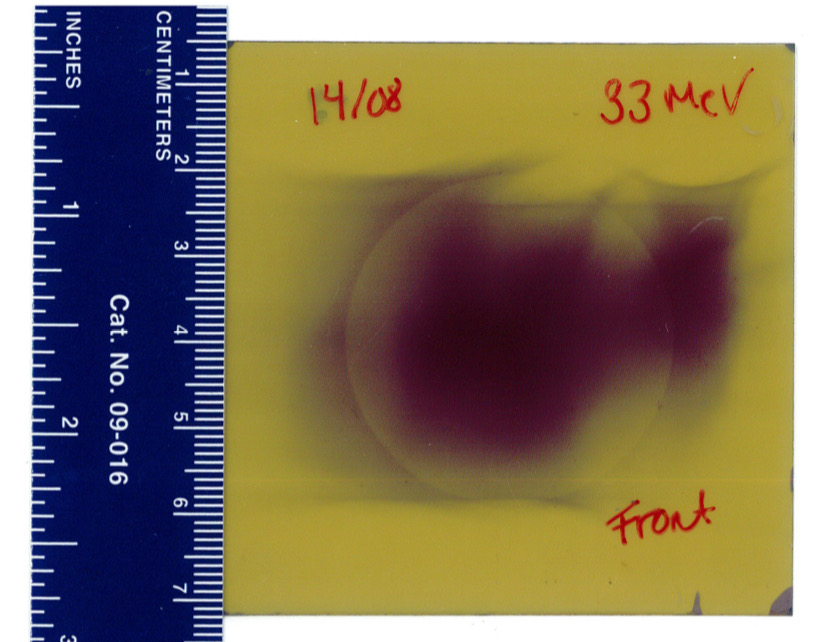
\includegraphics[width=1\linewidth]{33MeV_front.jpeg}
  \caption{A subfigure}
  \label{fig:sub3}
\end{subfigure}%
\begin{subfigure}{.5\textwidth}
  \centering
  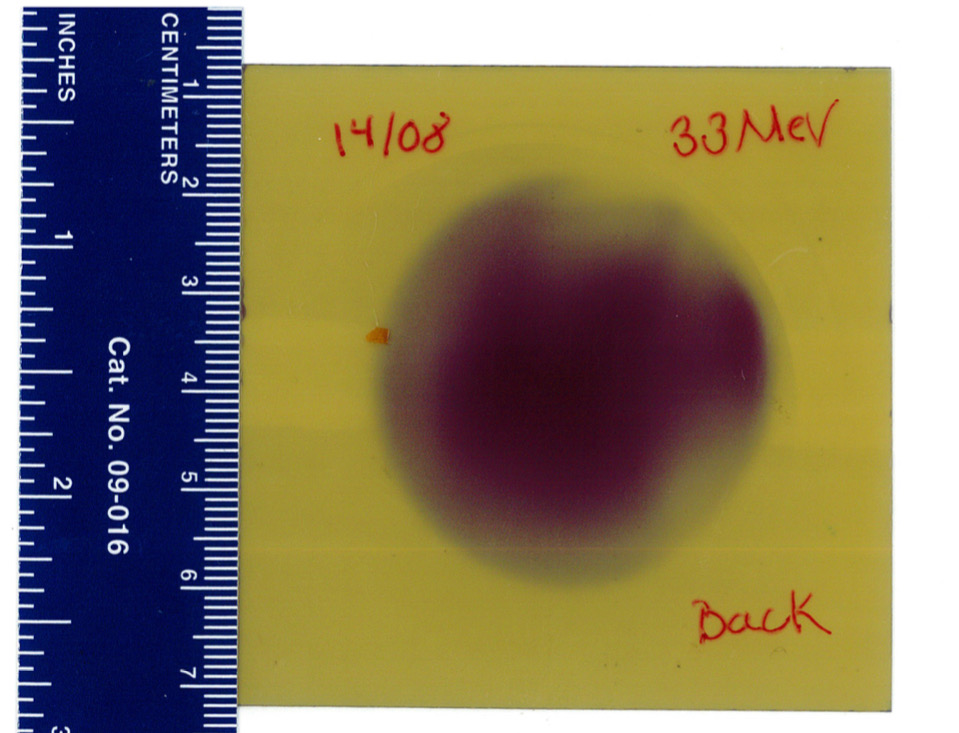
\includegraphics[width=1\linewidth]{33MeV_back.jpeg}
  \caption{A subfigure}
  \label{fig:sub4}
\end{subfigure}
\caption{Pictures of the beam shape. (a) and (b) shows the beam during the 16 MeV run, and (c) and (d) shows the beam for the 33MeV run.}
\label{fig:test}
\end{figure}
\noindent
After the the tuning, the targets were placed in a metallic box, see figure \ref{fig:target_stack}, and then placed in a tube that were sealed with vacuum. The vacuume were there to decrease the amount of interactions between the air prticles and the charge particle inside the targetholder. 
\\
\\
When the irradiation was done, the targets were removed to the counting room where they were placed in a gernanium detector \textcolor{red}{see section???}. 

\subsection{The 88-Inch cyclotron}
\label{sec: cyclotron}

Being one of the first cyclotrons used to produce medical isotopes \cite{E.Lawrence}, the Berkeley lab is still used to produce radionuclides that are a part of the research in the medical industry. Lawrence national laboratory is located in the hills, directly over the university of California at Berkeley overlooking San Francisco bay.\\
\\
The 88-Inch cyclotron is used in research on varies of fields including astrophysics and nuclear structure. The accelerator is a 300-ton, K = 140 sector-focused cyclotron with the ability to run with both heavy and light ions. The K-value represents the kinetic energy a particle can reach in the cycotron and can be used to rescale the energy reach for protons to other charge-to-mass ratio $E_k = A K (\frac{Q}{A})^2 $. Where A is the change in atomic mass, Q is the amount of energy released in a reaction and $E_k$ is the kinetic energy to a proton.\\
The facility of the cyclotron is shown in figure \ref{fig:Control-Room-Map}, it mainly has five experimental caves where cave 0 is the one used for neutron beams and isotope production. \textcolor{red}{The cyclotron can accelerate ions up to 70 MeV}  ...
\\
\\
- k-value (descuss energies for hospital cyclotrons and what energies for Cu64,67), what is it, how does it work\\
- no more than a page or two (look at other theses o se how deep you should go)

\subsection{Deuterium breakup prosess}
\label{sec: D_breakup}

Since a neutron beam has to be created, the usage of deuterium to make neutrons was done by  thick target deuterium breakup. This prosess has been studied by Meulders \cite{Meulders} and Saltmarsh \cite{Saltmarsh1977} and it involves splitting up deuterium into a proton and a neutron using a thick target of beryllium.
\\
\\
Deuterium break up can be done on any material but natural beryllium is a dense medium that has the quality as a good conductor of heat, it is stable and it is impossible to produce a radioactive activation product using deuterium. Be has a low Z wich means that the atom dencity is lower and as a result, the breakup yield will increas.  There is no excited states in deuterium \cite{deuterium_decay} and because of the low binding energy of 2.22 MeV it will easly split into one proton and one neutron when it hits the beryllium target with energy greater than the bindng energy of the deuterium.

\begin{figure} [h!]
   \centering
   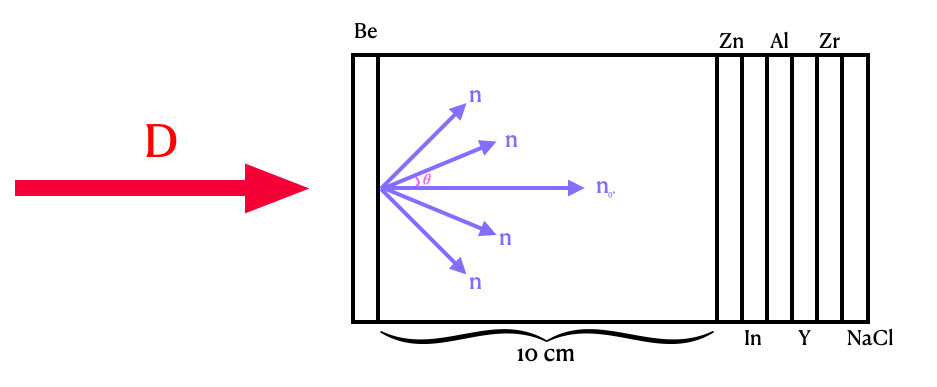
\includegraphics[width=1\linewidth]{D_to_n}
   \caption{Illustration of the deuterium breakup and how the neutron beam is dependen on the angle it gets emittet by.}
   \label{fig:D_to_n}
\end{figure}
\noindent
Deuterium breakup reaction can happen in two ways: direct process and excitation of the deuterium. The first one happens at higher energy where a proton interacts with an atom or the  electron cloud in the be target and strips off the proton, allows the neutron to pass through the beryllium disk.  At lower energies there are a probability to excite the deuterium. If the deuterium is being excited above the binding energy, there will be a coumpound nucleus and it will decay by sending out a proton or a neutron. The energy distribution of the neutron beam is visulized in fig \ref{fig:meulders_energydistribution} where the neutron flux increases with materials that have lower atmoic number. This is one of the main reasons to why beryllium was used in this experiment.

\begin{figure} [h!]
   \centering
   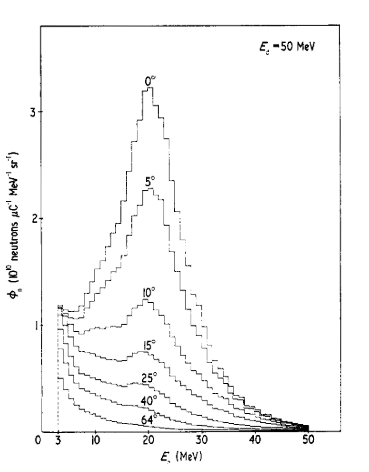
\includegraphics[width=.6\linewidth ]{zero_degrees_moulder.png}
   \caption{angles}
   \label{fig:angles_moulder}
\end{figure}
\noindent
\\
Fig \ref{fig:angles_moulder} shows how the energy varies with the angle of the neutron that is being emitted in the Be(d,n) reaction. When the angles of the neureons get bigger, the neutron flux decreases \cite{Meulders}. Even going from zero to ten degrees decreases the neutron flux by a factor if two. In this experiment the angles of the neutron flux were aimed to be zero degrees since the energy drops with the angle \cite{Meulders}. The assumption that the neuron flux spectra for 33 MeV and 16 MeV as fig \ref{fig:angles_moulder} is made with the knowlage that the energy will shif down. The expectation of an neutron flux energy of 16MeV deuterium beam is approximate 6.5 MeV and approximate 16 MeV for the 33 MeV beam. This is shown in fig \ref{fig:meulders_energydistribution}.

\begin{figure} [h!]
	\centering
	\begin{subfigure}{.5\textwidth}
  		\centering
  		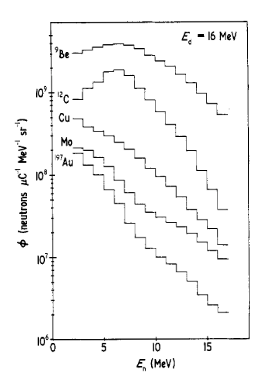
\includegraphics[width=.9\linewidth]{meulders_16.png}
  		\caption{A subfigure}
  		\label{fig:energy_16}
	\end{subfigure}%
  \begin{subfigure}{.5\textwidth}
    \centering
  	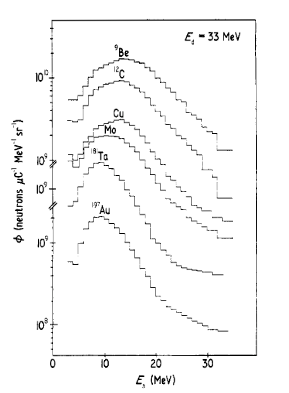
\includegraphics[width=.95\linewidth]{meulders_33.png}
  		\caption{A subfigure}
  		\label{fig:energy_33}
	\end{subfigure}
 \caption{Neutron energy spectra produced with 16 MeV in (a) and 33 MeV in (b) that were produced in the (d,n) reaction. Taken from \citep{Meulders}}
 \label{fig:meulders_energydistribution}
\end{figure}
\noindent




\subsection{Stack design}
\label{sec: stack_design}

A specific design of the targets were used to make sure that the cross section for each target could be measured for the different energies we iradiated the targets with. Five different targets, Al, In, Y, Zn, and Zr, were made into small “packings” using kapton tape to tightly seal them( see figure \ref{fig:target_design}), \textcolor{red}{ bruker dette også til å hinde contamination siden targetset kan være sjør og unngå spredning av løst radiaktivt stoff. }
\begin{figure} [h!]
   \centering
   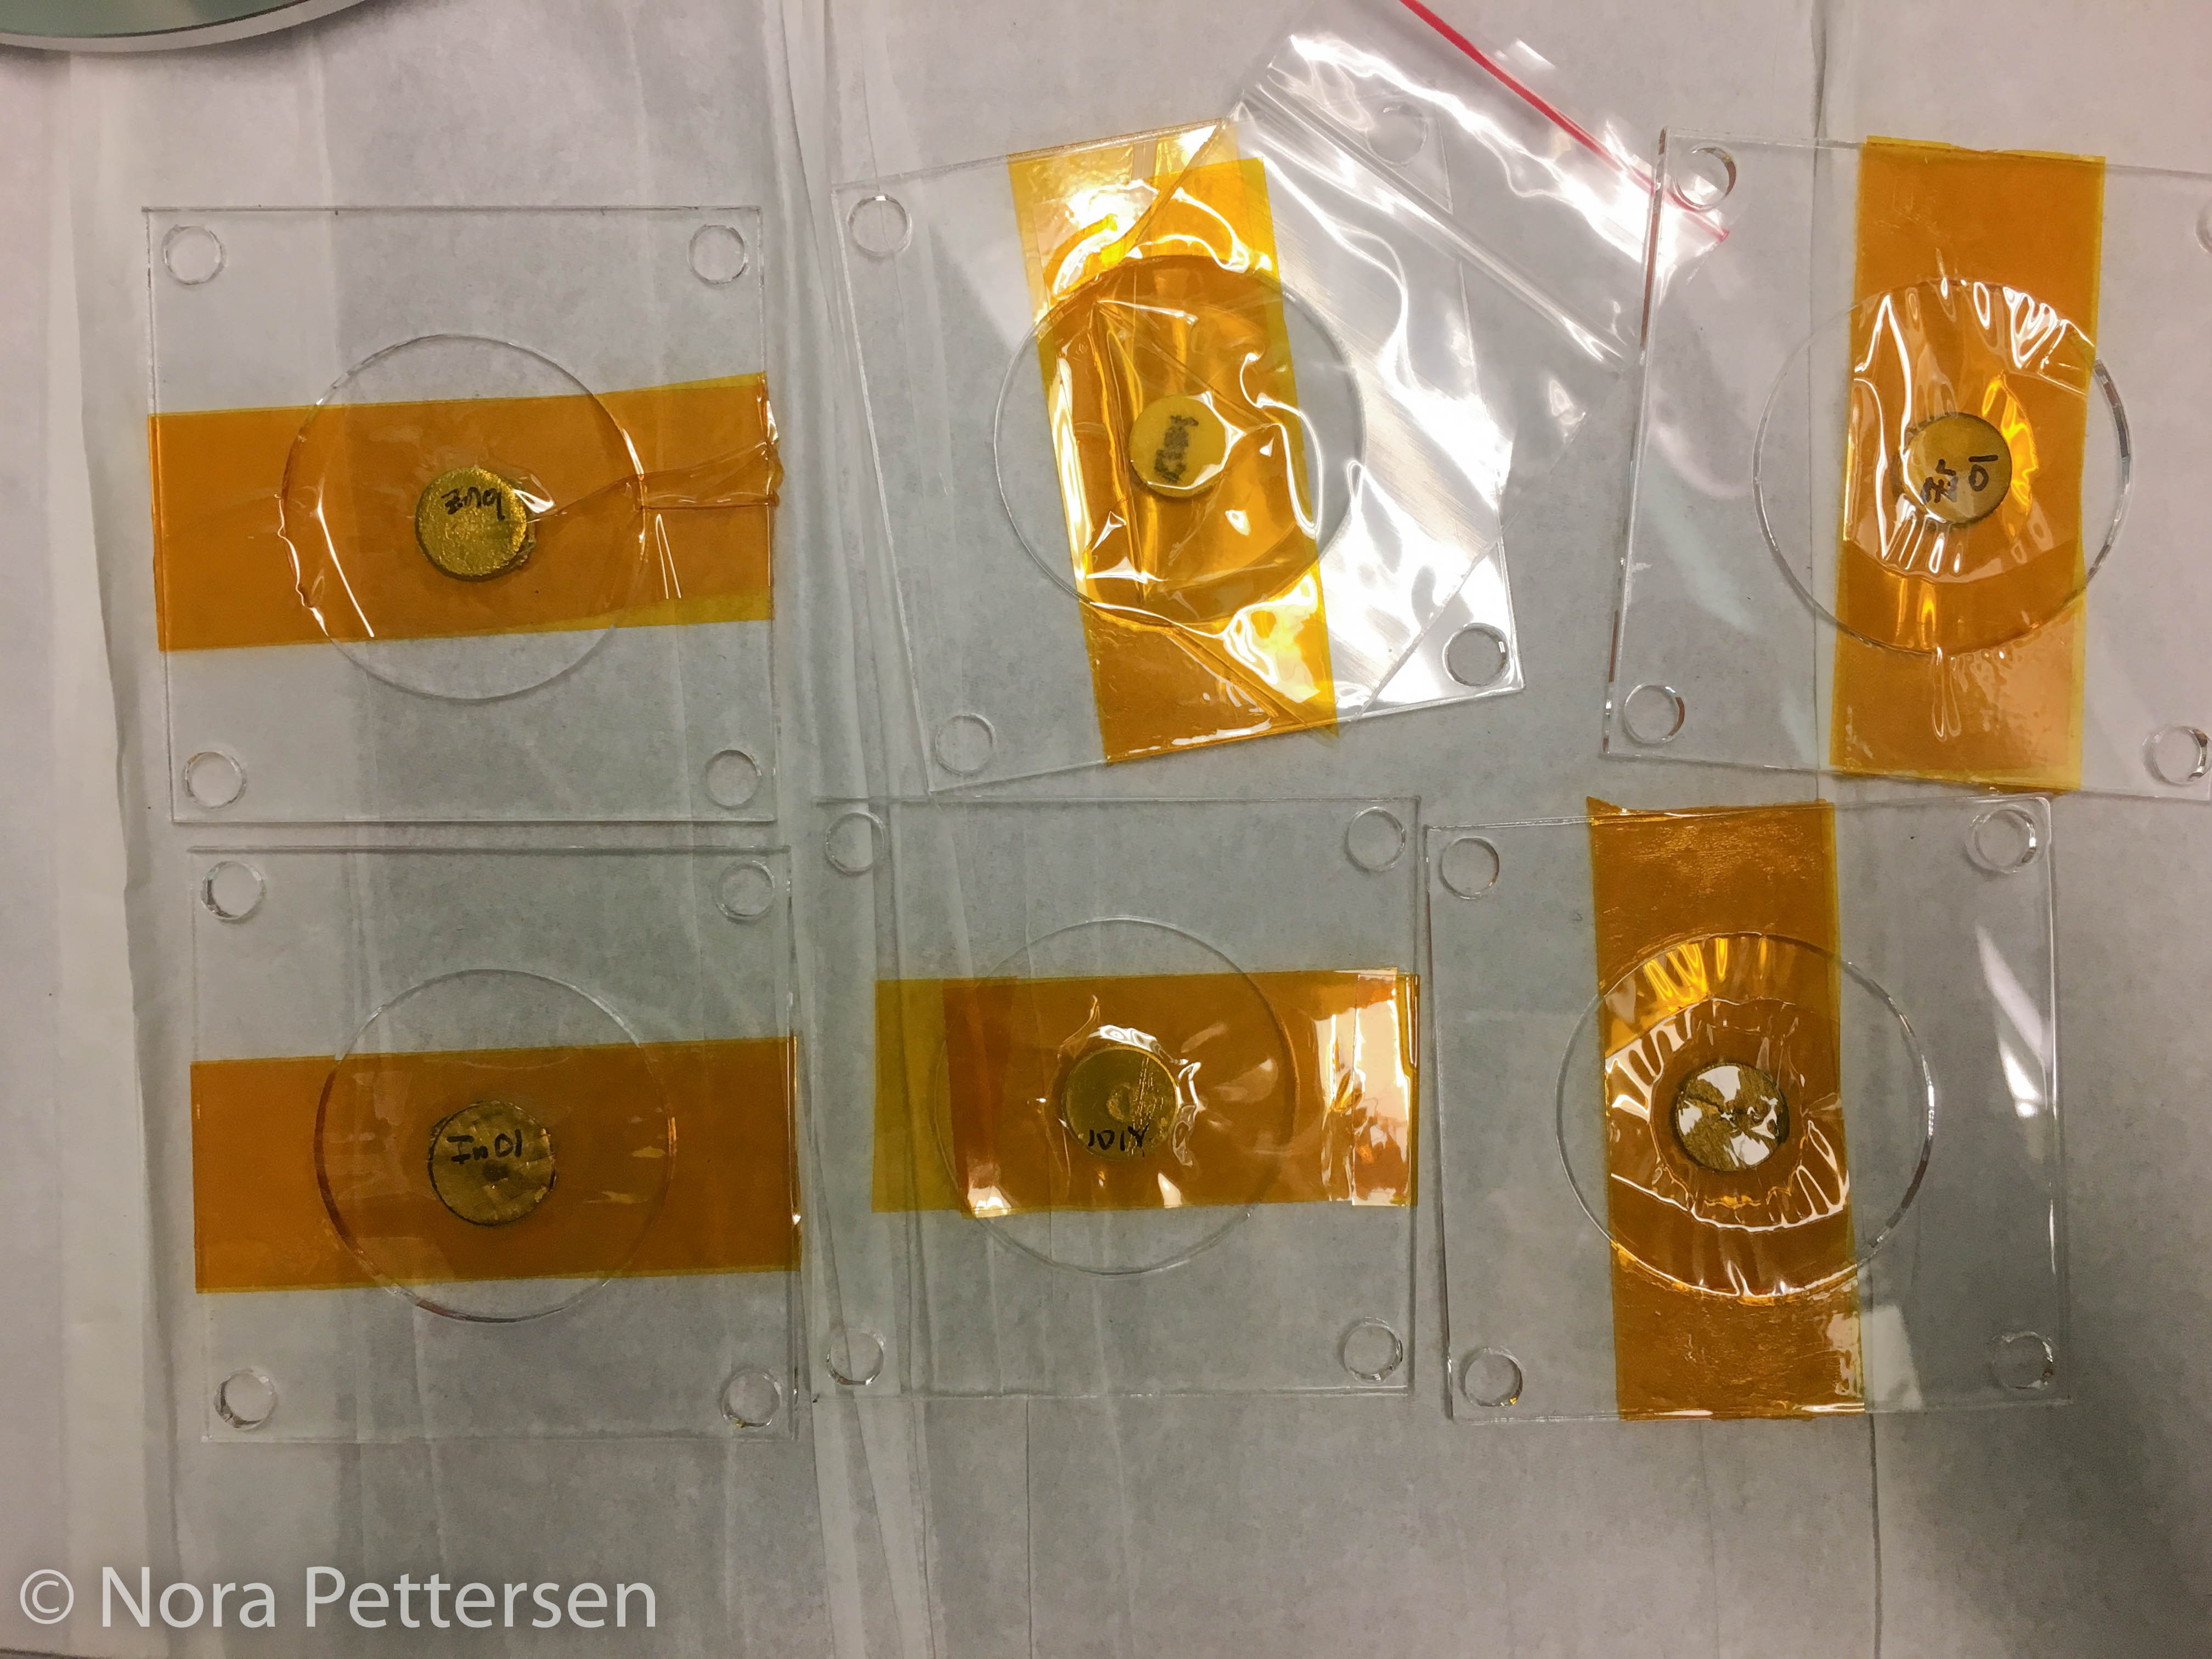
\includegraphics[scale=.2]{packs-1.JPG}
   \caption{Picture of how the targets were sealed before irradiation}
   \label{fig:target_design}
\end{figure}
\\
\noindent
The kapton contains polymer carbon, hydrogen and oxygen but the sticky part of the tape are made from silicone. For each target we measured their wight, thickness and length \textcolor{red}{Using what?} to calculate the uncertainty of each target. The targets were attached to a plastic frame and were placed in the end of a metallic \textcolor{red}{box made of?} where we wanted the targets to be 10 cm from the Br disk, the targets were held in place by a spring between them and the disk in front. 
\begin{figure} [h]
   \centering
   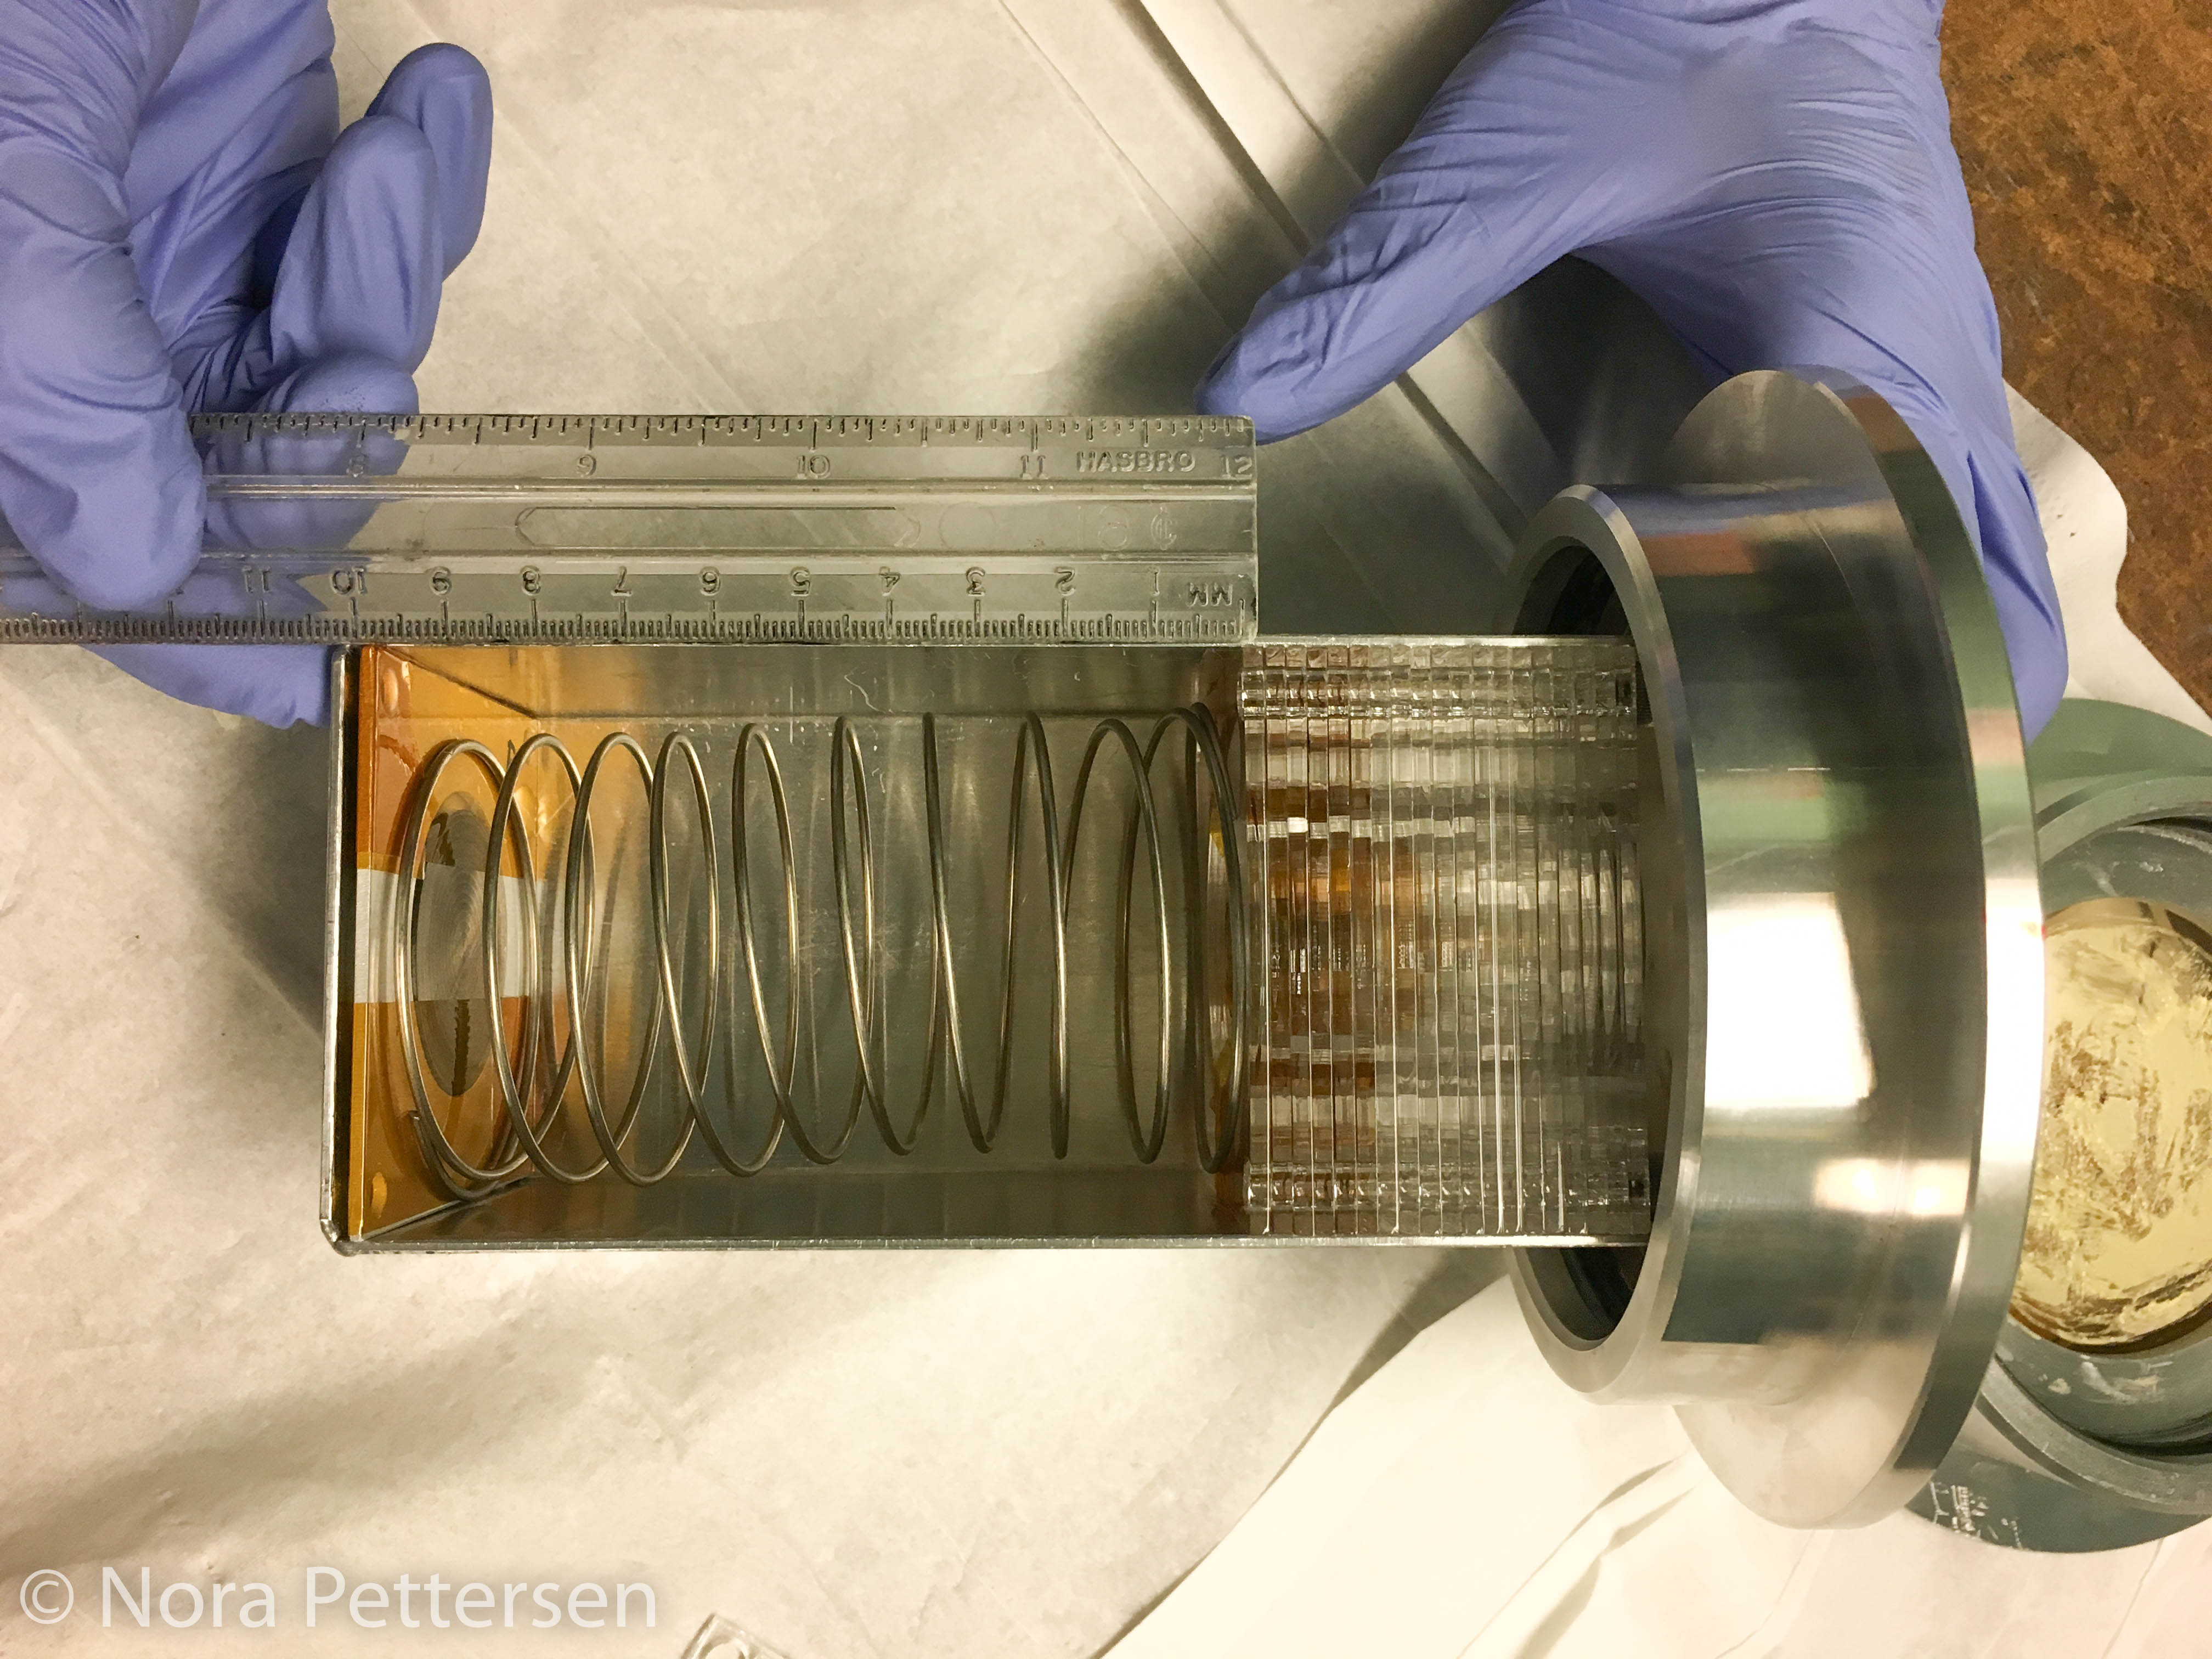
\includegraphics[scale=.2]{target_stack-1.JPG}
   \caption{Picture of how the targets were placed in the metallic box before irradiation}
   \label{fig:target_stack}
\end{figure}
\\
\noindent
The metallic box was then placed in the beamline by inserting it into a vacuumous tube. The vacuum was there to prevent the beam to hit air molecules and to make the beamline as straight as possible, such that more of the beam would be able to hit the targets. The radiation of the targets were on for approximately \textcolor{red}{12 hours?} for both 16 MeV and 33 MeV. 
\cite{E.Lawrence}


- photos and stuff\\
- monitor foils



\section{Radiation}
\label{sec:radiation}


- beam monitor to meassure the  \\
-- plot the beam current  as a function of time to justefy thet we can make the math that we do


\subsection{Counting}
\label{sec:counting}

- after each radiation, we removed the foils to the counting room (how long did this take?) hvor lang ti tok det før vi begynte å telle etter EOB?


\section{Gamma spectroscopy}
\label{sec: gamma_spectro}

- Detector, ortec gmx detector\\
-- forklare hvor dypt jeg skal gå inn i physics (doping, n-p junktion)\\


\subsection{Gamma spectra}
\label{sec: gamma_spectra}

- deadtime, og alt det der

\subsection{Calibrating}
\label{sec: calibrating}

- detectror efficincy\\
- curves at different position

% ----------------------------------------------------------------------------------------------------------------------
% ----------------------------------------------------------------------------------------------------------------------

\chapter{Analyse}
\label{ch:analyse}

\epigraph{\itshape ``If you ever start thinking too seriously, just remember that we are talking monkeys on an organic spaceship flying through the universe"}{--- \textup{Joe Rogan}}



\section{Fitz peak}
\label{sec:fitz_peak}

FitzPeaks Gamma Analysis and Calibration Software is a program that  is being used for gamma spectroscopy analysis and calibration. The program uses linear least square routine \textcolor{red}{DESCRIBED WHERE?} and tries to fit the data to a gaussian function. 
\\
 \\
- Data to activity ( the math). Peak counts to activity\\
- i - Aktivity to A$\_$EOB\\
- Production physics (Analyse eller Resultater?) - how we calculate cross-sectrtion, the work with john to use the monitor data to neutron fluxes that I’m going to use for calculate the cross section for my isotopes



\subsection{Regression prosess}

$\chi^2$- distribution is a set of distibution depending on how many sets you have 
\\
- non linear regression

\section{Production physics}
\label{sec: prod_physics}

Activity is written as $$A(t) = A_0 e^{-\lambda \Delta t_{decay}}$$
And that deca0ys with $$\Delta D = \int_{t_{live}}^{t1} A_0 e^{-\lambda t} dt = \frac{A_0}{\lambda} (1- e^{-\lambda \Delta t_{live}})$$
Efficiency is then $$\epsilon_{eff} = \frac{N_c}{\Delta D I_{\gamma}}$$ where $N_c$ is the number of counts.
The efficiency then becomes $$\epsilon_{eff} = \frac{\lambda N_c}{A_0 I_{\gamma} (1 - e^{-\lambda \Delta t_{live}}) (e^{-\lambda \Delta t_{decay}})}$$


$A_0$: $$A_0 = N_T \cdot (1-e^{-\lambda t}) \cdot \int \sigma(E) \frac{d\phi}{dE} dE$$
\\
Average cross section: $$\sigma_{avg} = \frac{A_0}{N_T (1-e^{-\lambda t}) \cdot \phi_{avg}} $$
\\
\
From deuterium to neutron energy:
\\
$$E_{avg} = \frac{\int E \cdot d\phi(E)}{\int d\phi ( E)} $$ 
where $d\phi dE$  is the energy dependent neutron flux.
\\
\\
To find the errorbars in the neutron energy a calculation of FWHM of $\frac{d\phi}{dE}$ form the meulders paper\cite{Meulders}. A list of energies and a list of the $d\phi dE$ is being plotted where the maximum value of the neutron flux is collected. \textcolor{red}{INCERT FIGURE OF MEULDERS} The half of the maximum value is being used to find the intersection between $E_n$ and $d\phi dE$ wich gives two energy values, $x_1$ and $x_2$. To find the errorbars $\delta E$ of the neutron flux these equations are ben gused.
$$E_{x_1} = E_{avg} - \delta E_{lower}\hspace{.5cm} , \hspace{.5cm} E_{x_2} = E_{avg} + \delta E_{upper}$$ where $\delta E_{lower} \neq \delta E_{upper}$ because $\frac{d\phi}{dE}$ is not symmetric, as shown in fig\ref{}

% ----------------------------------------------------------------------------------------------------------------------% ----------------------------------------------------------------------------------------------------------------------

\chapter{Results and dscussion} 
\label{ch: res_and_discussion}
- Cross sections for all the isotopes\\
- experimentall data with the data that has been meassured so fare


\section{TALYS}
\label{sec: talys}


- tolking av resultat. Hvilke energier er best i forhold til hva vi ser?\\
- Verdien av dette i fremtiden?\\
- how can we  desien target for å kunne produsere mer Cu67. hvilke cyclotrons can we use for that? 

\section{ALICE}
\label{sec: alice}

\section{EXFOR}
\label{sec: exfor}


% ----------------------------------------------------------------------------------------------------------------------% ----------------------------------------------------------------------------------------------------------------------




\chapter{Summary and outlook}
\label{sum_and_outlook}
\section{Future work}
\label{sec: future_work}


\epigraph{\itshape quote}{--- \textup by }

% ----------------------------------------------------------------------------------------------------------------------% ----------------------------------------------------------------------------------------------------------------------

%\begin{appendices}
%\chapter{Some Appendix}
%The...

%\blindtext


%\chapter{Some other appendix...}
%\blindtext

%\end{appendices}


%\bibliographystyle{unsrtnat}
%\bibliographystyle{mybibstyle} %my own bibstyle to set first names to one letter + unsrtnat
\bibliographystyle{IEEEtran}
%\bibliography{library.bib}

%\bibliography{/Users/ikkullma/Documents/MendeleyDesktop/Oslo_Method.bib,web_references.bib,other_ref.bib,/Users/ikkullma/Documents/MendeleyDesktop/GeneralNuclearPhysics.bib,/Users/ikkullma/Documents/MendeleyDesktop/NuclearAstro.bib}

%change the user...
\bibliography{/Users/Nora/Documents/UiO/Masteroppgaven/Oppgaven/library.bib}


\end{document}